\chapter{Conclusions \& Future Work: Opportunities for Fostering Creative Learning}
\begin{quote}
    My hope is that this dissertation has demonstrated that attunement benefits creative exploration because knowing how to ``see'' is central to expertise. While simply telling people may not be sufficient (Section \ref{sec:hats_exp}), I believe that richer attunement scaffolds can be highly effective. For example, this dissertation presented a simplification attunement scaffold to help people focus on high-level visual composition (Chapter \ref{chapter:abstraction}), a scaffold for presenting conceptually-relevant examples (Chapter \ref{chapter:shown}), and a scaffold for reusing high-quality examples in improving feedback (Chapter \ref{chapter:critiquekit}). This chapter describes opportunities for future work with these scaffolding strategies.
\end{quote}

\section{Embracing Ambiguity}
I believe that a major roadblock to exploration and creative work is an emphasis on perfection or quantifiable metrics rather than iteration and progression. Creative work by nature is ambiguous, which makes fixating on the salient and the concrete all the more appealing, an ``analysis paralysis'' or choice paradox where so many options are possible that satisficing on one seems like the best solution to avoid being wrong \cite{grant2021think,schwartz2004paradox,simon1972theories}. Part of developing expertise is learning what details to pay attention to and when and not getting lost among the `trees.' For instance, focusing on the perfection of a character's outfit while sketching early on can distract (literally) from the bigger picture. Representations work best when the amount and type of expression they facilitate align well with the goal. One benefit of expertise is being able to break down the larger problems into simpler chunks where novices have greater difficulty in seeing how to do so. Abstraction blocks make concrete the intangible, abstract things that are easy to overlook. We found that groups using abstraction blocks in drawing focused more on composition concepts rather than details like what color a coat should be (Section \ref{sec:abs_study}). The key insight of abstraction blocks is that they make the ambiguous visible and tangible, emphasizing exploration rather than settling on the first known idea. Our study looked at abstraction blocks as an aid for chunking in drawing. Groups that used abstraction blocks formed composition plans with post-it notes as blocks (Figure \ref{fig:abs_drawings}). Abstraction blocks enabled top-down thinking, forming the plan before executing on the details. This draws similarities to backwards design in learning where the overall goal determines the plans and means to achieve that goal \cite{wiggins2005understanding}. 

Setting high-level goals in creative work is difficult because the details distract us in two ways: 1) we do the small stuff to procrastinate from the tougher stuff, and 2) we get so focused on making the small stuff `right' that we can't get past it. I believe the abstraction blocks approach can work domain-generally to help people set high-level goals by removing the details that distract and pigeonhole us.
For example, in writing, focusing too heavily on grammar or wording early on can distract from the high-level narrative and flow of the writing \cite{sommers1980revision}. Abstraction blocks for written work might first start out with blocks for general plot points (\textit{i.e.} conflict and resolution or character development) before the writer begins composing sentences for each block. At an even higher level, what might abstraction blocks look like for making life decisions, like financial planning or figuring out career plans? Can these high-level goals be `chunked' in a way that decomposes the details?

\begin{figure}
\centering
  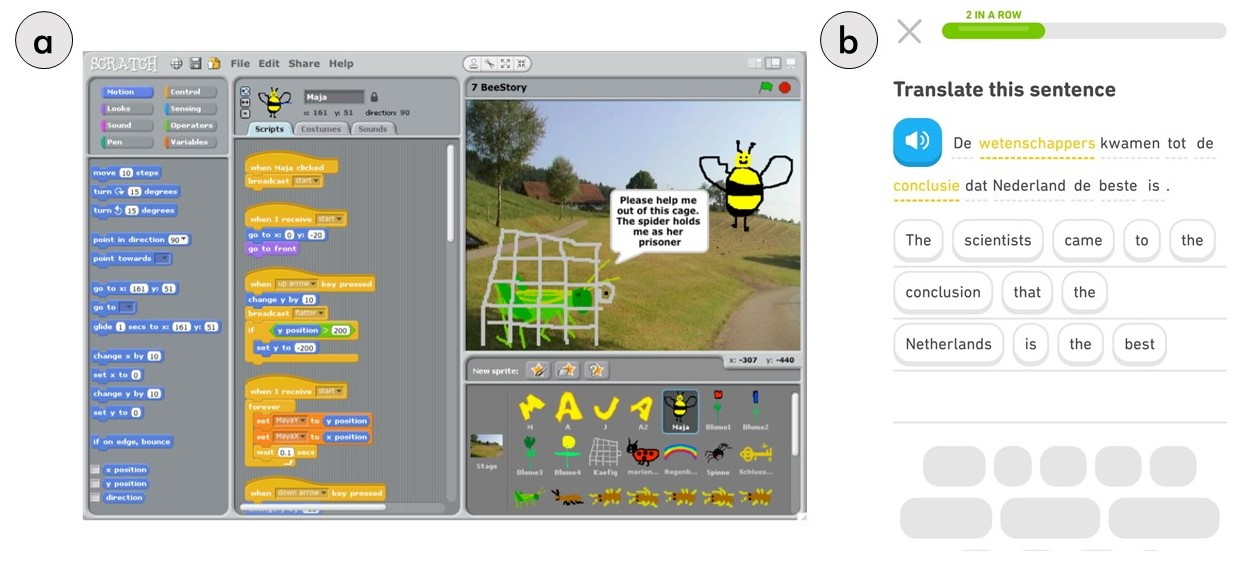
\includegraphics[width=\textwidth]{i_figures/blocks.jpg}
  \caption[Similar to the concept of abstraction blocks, Scratch \cite{Resnick2009} uses block-based programming --short phrases visually rendered into discrete, parameterized blocks-- to help novices easily create games and programs]{Similar to the concept of abstraction blocks, a) Scratch \cite{Resnick2009} uses block-based programming --short phrases visually rendered into discrete, parameterized blocks-- to help novices easily create games and programs by understanding the higher-level concept without worrying about syntax or technical coding details. b) Duolingo \cite{von2013duolingo}(www.duolingo.com) uses blocks to help learners build and translate sentences without the need for minor spelling or grammar concerns.
}
  \label{fig:scratch}
\end{figure}
%make both scratch and duolingo and clearer what the blocks are. In scratch, short phrases visually rendered as discrete, parameterized blocks...in duolingo, blocks to form sentences.

We can look to systems that already use a form of abstraction blocks. Scratch \cite{Resnick2009} and Duolingo \cite{von2013duolingo} incorporate ``blocks'' as physical and moveable instantiations of coding or language learning to make learning more tangible (Figure \ref{fig:scratch}). In our study, abstraction blocks made drawing almost like a puzzle, allowing groups to put the pieces together to create their picture. Finding ways to chunk problems into blocks and scaffolding the process of ``assembling'' them is a promising direction for creativity support tools. For example, tools could provide ``levels,'' where users can toggle between more abstract, malleable chunks and more concrete detailed levels so they can easily shift between exploring the ambiguous and making concrete decisions on the details. Future work should examine how abstraction blocks might be applied as an oblique strategy for scaffolding attention to high-level plans and goals. 

\section{Meeting People Where They Are}
The big vision in education more generally is taking less of a `one-size-fits-all' approach and more of a personalized style to teaching and learning. Someone entering my Cognitive Science graduate program with a mathematics background is going to have a different knowledge base, skillset, and goal than someone with a psychology background, for instance, and the form of training and learning that works best for these two students will look different. The studio-apprentice model and one-on-one tutoring best exemplify this approach where help is adapted to individual learners \cite{bloom1984,Chi2001,schon1984reflective}. In Sch{\"o}n's architecture scenario, the expert explains in detail the choices he makes to the student and engages in a Socratic dialogue \cite{schon1984reflective}. Tailoring learning to one's individual knowledge and goals is tractable for the first time with computers. To emulate this dialogue, Sh{\"o}wn's adaptive conceptual guidance presents general examples to users depending on their actions (Chapter \ref{chapter:shown}). Sh{\"o}wn used predetermined heuristics to decide what conceptual examples to show and when. What if tools could adapt the heuristics to users? 

%prereqs as an example of failure of one-size-fits-all. Someone w/ math background going into phd program vs. psych background and having different goals. Tailoring learning to one's knowledge and goals is for the first time tractable with computers.
%we all come with different knowledge and perceptions, but people don't necessarily learn differently. Make clear 

Every user has individual goals; some want to learn the concepts and gain deliberate practice in a skill while others might want to quickly execute a task without worrying about learning the concepts. Future creativity support tools should provide the most appropriate help for these goals. From our observations with Sh{\"o}wn, we saw that proactive guidance gave novices an awareness of options to consider; user-led, reactive guidance was more useful for small, concrete tasks (Section \ref{sec:shown_exp}). User-led searches are great when you know what to search for, but it's the unknown unknowns that make productive search both unlikely and extremely challenging if you don't know with what you need help. This is where a good tutor, whether a professional or peer, can proactively direct attention to issues you may not have considered and provide new insights. To close the loop, tutors can offer a record of the skills you have mastered and give targeted help for your specific areas of improvement. Similarly, a well-designed adaptive computational tool could proactively suggest help as you need it and create a record of skills you've mastered. Just as a human tutor might give more or less help depending on a learner's progress, tools could also include different modes of help. For instance, a ``maximum help'' mode could provide the most guidance, both for conceptual understanding and technical skill help, while a ``minimum help'' or ``silent'' mode might provide only technical skill help or no help at all. These tools would give freedom to the user to decide which type of guidance they need depending on their own individual goals and tasks. 

%big DEI benefit of computational tutors, with luck, computational coaches can help minimize/counter shortcomings of differing backgrounds.
%A good TA or tutor can recognize which prereq is missing that can lead to another stumbling block. They realize the cause of the error.

\section{Creating Opportunities for Risk-Taking}
Even today, many people hold a folk belief that mathematical abilities are innate rather than learned or grown \cite{rattan2012s}. Similarly, creativity seems to be another attribute that people think of as an innate talent or something accrued through deep experience in a given field rather than in a structured, deliberate manner. This dissertation argues that structured attunement can at the very least catalyze creative exploration and learning. Exploration inevitably includes giving up on some ideas. Most early ideas do not succeed, and the feeling of ``wasting time'' can limit further exploratory efforts. However, wild or even bad ideas can lead to serendipitous discoveries \cite{osborn1953applied}. Creating low-stress and low-stakes environments can encourage exploration and risk-taking. Often, professional and educational settings engender an anxiety that makes people terrified to fail and therefore, terrified to take risks. Risk-taking requires that you can survive the failure. 

Part of taking risks is understanding what aspects are worth the risk and what aspects need iteration. Feedback is a critical piece of this puzzle, learning what works and getting a direction for where to go \cite{Hattie2007,sadler1989formative}. Our work with CritiqueKit showed that reusing exemplar feedback according to the structural critiera of being specific, actionable, and justified can improve feedback quality (Chapter \ref{chapter:critiquekit}). The next step is understanding how feedback is interpreted and applied. In human tutoring and studio models, experts use a variety of representations to explain concepts to a novice, such as sketches or deictic gestures like pointing \cite{goldin1999,schon1984reflective,Tversky2011}. To emulate how an expert might provide feedback to a novice, particularly for visual or multimedia mediums, future feedback tools could allow reviewers to directly demonstrate their suggested improvements through multimodal and deictic interactions. Similar to how ReMap \cite{fraser2020remap} uses deictic gestures and speech queries to find relevant moments in videos to present to users, feedback tools could also use these interactions as context to search for appropriate feedback suggestions from a corpus of critique examples. I hope the direction of critique tools help people both give feedback and better apply it to their work to give people the safety and freedom to take risks in their creative thinking.

% One strategy is to visually show common areas of critique to highlight priorities and show contradicting feedback from reviewers  \cite{yen2020}.

% Capturing good expert and peer feedback and reusing exemplar feedback can foster this community of critique where progression and improvement are emphasized rather than simply achieving a final outcome. 
% Systems like CritiqueKit that reuse previous feedback and scaffold effective and efficient feedback-giving can promote formative improvement rather than summative evaluation \cite{Head2017,Krause2017}. We found that adaptive and interactive feedback reuse drew attention to the structural characteristics of effective critique rather than just the content (Section \ref{sec:critiquekit_exp}).
 
\section{A Future for Computational Coaching}
A few years ago I began working with a boxing coach to improve my proficiency and technique with the goal of sparring more advanced students. My coach saw that despite my smaller size, I have quick footwork, sharp punches, and good handspeed. He tailored his coaching to improve my weaknesses in a way that capitalized on my strengths and showed me alternative ways to handle potential scenarios during a sparring session. Good coaches do exactly this: tailor their efforts to the individual learner and helping them hone their own style. I believe the future of creativity support tools is to emulate coaching, giving people the strategies and tools to accomplish their goals and improve. The future directions I've laid out in this chapter present opportunities to bring us closer to my vision. While this dissertation and other work within creativity support focus on digital learning and creation, an exciting area for computational tools and coaching is in physical domains like woodworking or dance. This dissertation presented three strategies that form the basis for what future computational coaching tools in any domain might become. These tools should provide attentional scaffolding to high-level concepts, adaptive support and relevant examples, and actionable feedback for improvement. We can learn skills and concepts from resources like video tutorials or books, but I believe that learning how to handle open-ended problems and ambiguous scenarios can come from adaptive and interactive guidance from contextualized, personal coaching.

\begin{figure}
\centering
  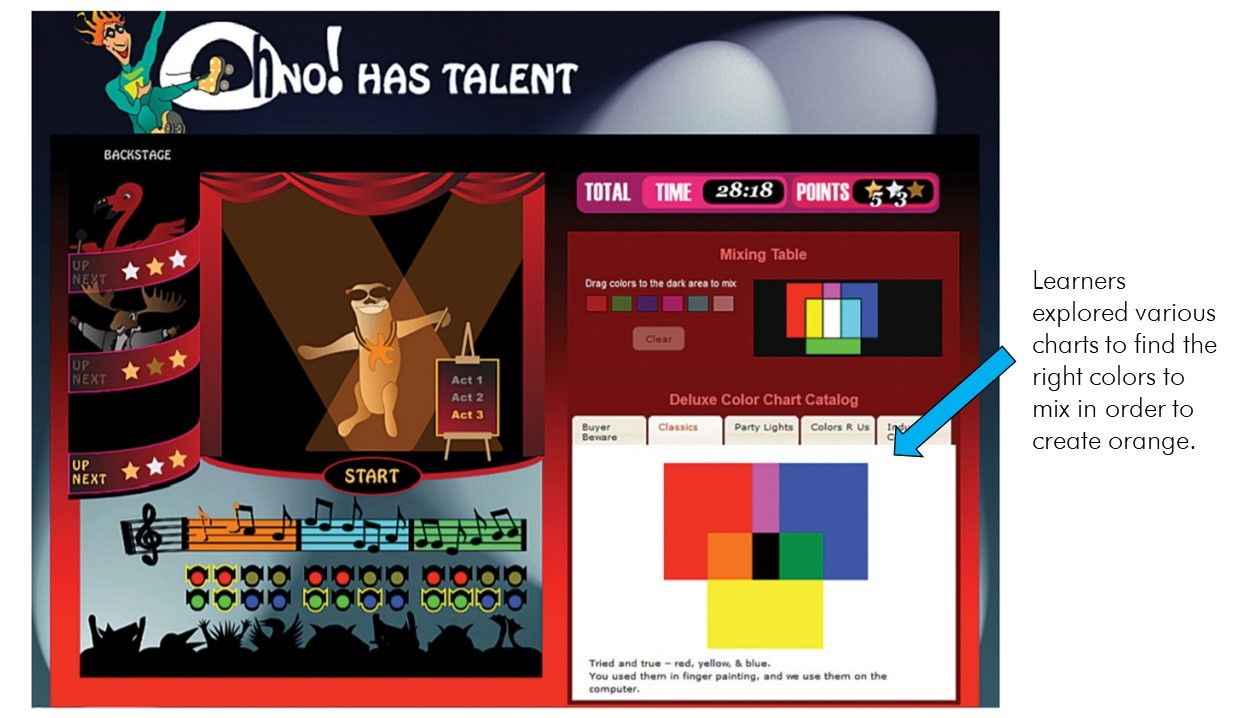
\includegraphics[width=.9\textwidth]{i_figures/choicelet.jpg}
  \caption{Ohno! Has Talent is a choice-based assessment of critical thinking ability where students can explore different charts to decide which ones give the correct information for mixing the intended color (orange). If they create mix the colors correctly, Ohno! will begin singing. Figure adapted from \cite{schwartz2013measuring}.
}
  \label{fig:choicelet}
\end{figure}
%add overlay of figure w/ arrow to point out the learning goal, add in the critical thinking piece for caption. 

One promising avenue for adaptive coaching tools are those that assess motivation and choice. Choice-based assessments and activities examine what choices learners make such as whether they choose to explore resources or try different potential solutions \cite{schwartz2013measuring}. Figure \ref{fig:choicelet} shows an example of a `choicelet' where students can choose to examine a catalog of color mixing charts to determine which charts are correct for their task as an assessment of critical thinking. Much like a human coach, computational coaches could help learners make and evaluate their choices could improve creative learning. In our study with Sh{\"o}wn, we found that some participants in our study wanted to understand more about the reasoning behind suggestions and how the examples could apply to their own comics (Section \ref{sec:shown_exp}). In addition to presenting suggested considerations, adaptive systems like Sh{\"o}wn could also provide explanations for why those considerations might improve a user's work. Many creativity support systems have toolbars that give users a variety of options of tools to user to execute their goals. What if coaching systems had ``strategy bars'' that allowed users to select different high-level strategies to use? This approach would give users a way to quickly explore different methods of achieving their goals and finding the strategy that works best for them.

Good coaches are few and far between, but the benefits of a coach are immeasurable. Issues of access and opportunity prevent some from even being able to afford to pursue their creative desires. Computational support tools could scale the talent of valuable coaches to nearly anyone who wants to learn. I believe that computational coaching tools should give opportunities to explore and connect exploration to their ultimate outcomes, meeting people where they are and helping them define and achieve their goals. I don't think computers should replace people's creativity, nor do I think they can. Rather, I see computational tools as a way of broadening people's horizons so they can accomplish more than they believe is possible.

\section{Closing Remarks}
Our information-driven society comprises an abundance of uncertainty, ambiguity, and information, in which we can often get lost in the woods. It is increasingly tempting to “cool” too soon, settling on
what little certainty we can find. Without “seeing the forest for the trees,” we may never come upon innovative solutions for our most complex problems. My dissertation introduces three strategies that help overcome this challenge. It contributes three interactive and contextual tools that embody these strategies to adaptively scaffold exploration at different stages of the creative process. It provides empirical evaluations and observations to demonstrate the efficacy of these strategies. Finally, the strategies introduced in this dissertation provide direction for open questions of fostering creative learning and scaling computational coaching to catalyze creativity for all. 
Ultimately, I envision a future in which our pedagogy and support tools empower people to practice everyday creativity to achieve their goals and expand human ambition.

%how do computational coaches mix w/ backwards design
%worth considering dual-ended search (how keen am i? how bad do i need to know it?), do convolution of those 2 things.
%socio-emotional factors, one challenge for forest for trees challenge is flying too high (icarus vs. fear of icarus), especially when collaborative (hard to figure out how to give and receive constructive criticism), pulling the plug on something.
